\documentclass[12pt,a4paper,twoside]{book}

\usepackage[spanish, es-tabla]{babel}
\usepackage[utf8x]{inputenc}

\usepackage[table]{xcolor} % para poner color en las tablas

\usepackage{tikz} %Gráficos
\usetikzlibrary{calc}
\usetikzlibrary{arrows,shapes,positioning,shadows,trees}

\usepackage{amsmath} % formulas sin numero
\usepackage{float}
\usepackage{hyperref} % habilita los hipervinculos

\usepackage{subcaption} %Varias imágenes, misma linea
\usepackage{graphicx} % para poner dos imágenes juntas
\graphicspath{{pictures/}{../pictures/}}
\usepackage{svg}


\usepackage{anysize}  %margenes
% MÁRGENES 
\marginsize{4cm}{2.5cm}{2.5cm}{2.5cm} 
%{izquierda}{derecha}{arriba}{abajo}

\usepackage{mathptmx}% http://ctan.org/pkg/mathptmx Times new roman
\usepackage{amsfonts}% Para expresiones matemáticas

\renewcommand{\baselinestretch}{1.5} % Interlineado
\usepackage{enumerate}% para los enumerate

\usepackage{fancyhdr} %header y footer
\pagestyle{fancy}

\usepackage[none]{hyphenat} %saltos y justificación texto

\usepackage{changepage} %margen y par/impar páginas

\usepackage{ragged2e} %Añade más funcionalidades de colocación de texto

\usepackage{listings} %Listas

\usepackage{appendix} %apéndice

\usepackage{color} %Colores

\makeatletter
\def\BState{\State\hskip-\ALG@thistlm}
\makeatother

%Ruta Imagenes

% COLORES
\definecolor{gray}{rgb}{0.4,0.4,0.4}
\definecolor{darkblue}{rgb}{0.0,0.0,0.6}
\definecolor{cyan}{rgb}{0.0,0.6,0.6}
\definecolor{palegreen}{rgb}{0.6, 0.98, 0.6}
\definecolor{palegoldenrod}{rgb}{0.93, 0.91, 0.67}

\colorlet{punct}{red!60!black}
\definecolor{background}{HTML}{EEEEEE}
\definecolor{delim}{RGB}{20,105,176}
\colorlet{numb}{magenta!60!black}


%Anexos Traducción
\renewcommand{\appendixname}{Anexos}
\renewcommand{\appendixtocname}{Anexos}
\renewcommand{\appendixpagename}{Anexos}

%Codigo fuente

\renewcommand{\lstlistingname}{Fragmento de código}

\lstset{
	basicstyle=\small\sffamily,
	numbers=left,
 	numberstyle=\tiny,
	frame=tb,
	tabsize=4,
	columns=fixed,
	showstringspaces=false,
	showtabs=false,
	keepspaces,
	commentstyle=\color{red},
	keywordstyle=\color{blue}
}

\lstdefinelanguage{json}{
    basicstyle=\footnotesize\ttfamily,
    numbers=left,
    numberstyle=\tiny,
    stepnumber=1,
    numbersep=8pt,
    showstringspaces=false,
    breaklines=true,
    frame=lines,
    backgroundcolor=\color{background},
    literate=
     *{0}{{{\color{numb}0}}}{1}
      {1}{{{\color{numb}1}}}{1}
      {2}{{{\color{numb}2}}}{1}
      {3}{{{\color{numb}3}}}{1}
      {4}{{{\color{numb}4}}}{1}
      {5}{{{\color{numb}5}}}{1}
      {6}{{{\color{numb}6}}}{1}
      {7}{{{\color{numb}7}}}{1}
      {8}{{{\color{numb}8}}}{1}
      {9}{{{\color{numb}9}}}{1}
      {:}{{{\color{punct}{:}}}}{1}
      {,}{{{\color{punct}{,}}}}{1}
      {\{}{{{\color{delim}{\{}}}}{1}
      {\}}{{{\color{delim}{\}}}}}{1}
      {[}{{{\color{delim}{[}}}}{1}
      {]}{{{\color{delim}{]}}}}{1},
}


\lstset{inputpath=code/, captionpos=b}
%Encabezado
\rhead{
    \begin{picture}(0,0) \put(0,0){
\includegraphics[width=1cm]{logo_uex.png}}
    \end{picture}
}

%Variables
\title{Sistema de indexación de palabras clave e identificación de voz en señales de audio}
\author{Pablo Macías Muñoz}
\def\tutor{Roberto Rodríguez Echeverría} % co-author
\def\cotutor{Juan Carlos Preciado} % co-author %configuracion


\begin{document}
\sloppy 
\pagebreak 
\makeatletter

\documentclass[../main.tex]{subfiles}
\begin{document}
\begin{titlepage}
	\begin{adjustwidth}{-1.5cm}{0cm}
		\begin{tikzpicture}[remember picture, overlay]
		\usetikzlibrary{calc}
		\draw[line width = 1.5pt] ($(current page.north west) + (1in,-1in)$) rectangle ($(current page.south east) + (-1in,1in)$);
		\end{tikzpicture}
		
		\vspace{-3.5em}
		\hspace{-0.5em}
		\begin{minipage}{0.45\textwidth}
			\begin{flushleft}
				
\includegraphics[width=1.75cm]{logo_uex.png}
			\end{flushleft}
		\end{minipage}
		
		\vspace{-6em}
		\hspace{20em}
		\begin{minipage}{0.45\textwidth}
			\begin{flushright}
				
\includegraphics[width=4cm]{logo_epcc.png}
			\end{flushright}
		\end{minipage}\\[1.5cm]
		
		\begin{center}
			
			
			% Upper part of the page
			\textsc{\LARGE UNIVERSIDAD DE EXTREMADURA}\\[4cm]
			
			\textsc{\Large Escuela Politécnica}\\[0.5cm]
			\textsc{\Large Grado de Ingeniería Informática en Ingeniería del Software}\\[3cm]
			\textsc{\Large Trabajo Fin de Grado}\\[0.5cm]
			{ \large \bfseries \@title}\\[4.0cm]
			\vfill
			% Bottom of the page
			{\large}
		\end{center}
	\end{adjustwidth}
\end{titlepage}
\end{document}

\pagestyle{empty}

\begin{titlepage}
	\begin{adjustwidth}{-1.5cm}{0cm}
		\begin{tikzpicture}[remember picture, overlay]
		\usetikzlibrary{calc}
		\draw[line width = 1.5pt] ($(current page.north west) + (1in,-1in)$) rectangle ($(current page.south east) + (-1in,1in)$);
		\end{tikzpicture}
		
		\vspace{-3.5em}
		\hspace{-0.5em}
		\begin{minipage}{0.45\textwidth}
			\begin{flushleft}
				
\includegraphics[width=1.75cm]{logo_uex.png}
			\end{flushleft}
		\end{minipage}
		
		\vspace{-6em}
		\hspace{20em}
		\begin{minipage}{0.45\textwidth}
			\begin{flushright}
				
\includegraphics[width=4cm]{logo_epcc.png}
			\end{flushright}
		\end{minipage}\\[1.5cm]
		
		\begin{center}
			
			
			% Upper part of the page
			\textsc{\LARGE UNIVERSIDAD DE EXTREMADURA}\\[3cm]
			
			\textsc{\Large Escuela Politécnica}\\[0.5cm]
			\textsc{\Large Grado de Ingeniería Informática en Ingeniería del Software}\\[2.5cm]
			\textsc{\Large Trabajo Fin de Grado}\\[0.5cm]
			{ \large \bfseries \@title}\\[4.0cm]			
			{ \large \bfseries Autor: \@author}\\[0.5cm]
			{ \large \bfseries Tutor: \tutor}\\[0.5cm]
			{ \large \bfseries Co-Tutor: \cotutor}\\[0.5cm]
			\vfill
			% Bottom of the page
			{\large}
		\end{center}
	\end{adjustwidth}
\end{titlepage}

\makeatother
\thispagestyle{empty}

%%%%%%%%%%%%%%%%%%%%%%%%%%%%%%%%%%
%%%%%%%%%% abstract %%%%%%%%%%%%%%
%%%%%%%%%%%%%%%%%%%%%%%%%%%%%%%%%%

\newpage
\thispagestyle{empty}

\documentclass[../main.tex]{subfiles}
\begin{document}

\chapter*{Resumen}\label{ch:es_abstract}
\thispagestyle{empty}
Los sistemas de reconocimiento de voz se encuentran en pleno crecimiento debido a la aparición de nuevas herramientas de inteligencia artificial y aprendizaje automático. Los sistemas más usados se encuentran online y son propiedad de las empresas más grandes a nivel mundial del sector TIC. Además ninguna de estas herramientas permite la adaptabilidad y mejora de modelos, despliegue personalizado y usabilidad por cualquier usuario. De esta necesidad nace este proyecto. 

Este documento describe el proceso seguido en el diseño e implementación de un sistema capaz de reconocer la voz en un audio, además de ser mejorable introduciendo más información, adaptable a cualquier entorno acústico, desplegable en cualquier servidor y usable por la mayoría de usuarios. 

Al finalizarse la lectura de este documento no solamente se entenderá la estructura del proyecto, sino que se conocerá la historia de los sistemas de reconocimiento de voz, cuáles son y en qué se basan las actuales herramientas que existen, qué objetivos cumple el sistema propuesto, qué tecnologías utiliza, cómo se ha desarrollado el proyecto y el resultado de algunas pruebas realizadas.

\smallskip
\noindent \textbf{Palabras clave.} lingüística computacional, voz a texto, entrenamiento de modelos, microservicios


\end{document}

\chapter*{Abstract}
\thispagestyle{empty}
EL RESUMEN EN INGLÉS

%%%%%%%%%%%%%%%%%%%%%%%%%%%%%%%%%%
%%%%%%%%%%% tablas %%%%%%%%%%%%%%%
%%%%%%%%%%%%%%%%%%%%%%%%%%%%%%%%%%

\pagenumbering{roman}
\setcounter{page}{1}
\tableofcontents
\newpage
\listoftables
\newpage
\listoffigures
\newpage


%%%%%%%%%%%%%%%%%%%%%%%%%%%%%%%%%%
%%%%%%%%%%% cuerpo %%%%%%%%%%%%%%%
%%%%%%%%%%%%%%%%%%%%%%%%%%%%%%%%%%

\pagenumbering{arabic}
\pagestyle{fancy}
\setcounter{page}{1}

\chapter{Introducción}
Esta plantilla sirve como ejemplo de TFG. Las secciones son las que están en la normativa. Esta sección la aprovechamos para introducir brevemente \LaTeX.

Algunos de los animales en peligro Figura \ref{fig:my_label} en la página \pageref{fig:my_label} extinción son el oso blanco\footnote{en el Ártico}, el cóndor\footnote{en los Andes}, el tigre siberiano\footnote{en Siberia}, y el lince ibérico\footnote{en la Península Ibérica}.

\begin{figure}
    \centering
    \includesvg[width=\linewidth]{flow_diagrams/flow_training.svg}
    \caption{Caption}
    \label{fig:my_label}
\end{figure}

\documentclass[../main.tex]{subfiles}
\begin{document}

\chapter{Objetivos}\label{ch:objetivos}
\section{Objetivo principal}\label{sec:obj_principal}
Descripción del objetivo principal
Indexación de palabras en un audio

\section{Objetivos secundarios}\label{sec:obj_secundarios}
Descripción de Objetivos secundarios
Aprendizaje del audio
Tratamiento del audio
Obtención de audio
Interfaz de comunicación

\end{document}

\documentclass[../main.tex]{subfiles}
\begin{document}

\chapter{Estado del Arte}\label{ch:estado_arte}
En este capítulo se describen los conceptos teóricos de la transcripción de audio, sistemas de transcripción de voz a texto existentes en el mercado y las alternativas tecnológicas para el desarrollo propuesto.
\section{Conceptos teóricos}


El reconocimiento del habla es una rama de la lingüística computacional que trabaja en desarrollar herramientas con las que una computadora traduce lenguaje hablado en texto. Esta tecnología puede recibir varias denominaciones: Reconocimiento Automático de la Voz (siglas ASR en inglés), Reconocimiento de Voz por Ordenador o Reconocimiento de Voz a Texto (Speech to Text en inglés). A lo largo de este documento también podrá encontrarse con la denominación de \textit{Transcripción de voz a texto}.

Dentro de los sistemas de reconocimiento de voz se pueden diferenciar dos grupos dependiendo del sistema de entrenamiento usado: por un lado existen los sistemas que analizan la voz de una persona leyendo un determinado texto para mejorar la precisión de la transcripción para ese determinado hablante (\textbf{sistemas dependientes del hablante}); y por otro lado existen sistemas que no necesitan entrenamiento por parte de una persona (\textbf{sistemas independientes del hablante}).

\subsubsection{Diferencia entre audio y sonido}

Durante esta documentación se mencionarán muchos términos relacionados con el audio y el sonido, por lo que es vital conocer la diferencia entre estas dos palabras:

En primer lugar, el sonido es una onda mecánica en forma de vibración que se desplaza a través de un medio de transmisión como un gas, un líquido o un sólido. Desde el punto de vista fisiológico humano, el sonido es la recepción de estas ondas mecánicas a través del oído y su transmisión al cerebro. Un ser humano de manera general puede oír ondas sonoras cuando la frecuencia de éstas se encuentra entre los 20 Hz y los 20 kHz. Si una onda sonora supera el umbral de 20 kHz se le denomina \textit{ultrasonido}, mientras que a las ondas sonoras inferiores a los 20 Hz se les conoce como \textit{infrasonido}. Cada especie animal tiene un rango audible de ondas sonoras.

Por otra parte, el audio es el sonido procesado por un sistema en las fases de grabación, transmisión y reproducción. A diferencia del sonido, que se capta por el sentido del oído, el audio se representa mediante una \textit{señal de audio} utilizando normalmente niveles de voltaje eléctrico (señales analógicas) o series binarias (señales digitales).

En este trabajo se analizará y procesará la voz humana que se encuentra en el audio. La voz humana consiste en el sonido que produce un ser humano utilizando su tracto vocal, mayoritariamente las cuerdas vocales. La relación entre las características del sonido y la voz son las siguientes:
\begin{itemize}
    \item \textbf{Intensidad}: Es el volumen con el que una persona habla. Esta intensidad o volumen se suele expresar en decibelios (dB).
    \item \textbf{Tono}: Es la característica que indica si una voz es aguda, media o grave. Está directamente relacionada con la frecuencia de las ondas generadas. Una baja frecuencia indica una voz grave, mientras que una voz aguda tendrá una frecuencia alta.
    \item \textbf{Duración}: Tiempo desde que un sonido se produce hasta que deja de hacerlo. En la voz se relaciona con la velocidad, ya que una persona que genere sonidos con menor duración al pronunciar una palabra, hablará más rápido que una persona cuya duración de sonido por letra o palabra sea mayor.
    \item \textbf{Timbre}: Es la propiedad que nos permite diferenciar un sonido con la misma intensidad, duración y tono pero producido por dos elementos distintos. En la voz, el timbre va a diferenciar entre dos personas emitiendo un sonido en la misma intensidad, el mismo tono y la misma duración. Esta cualidad se representa en ondas secundarias a la onda principal de la voz, llamadas armónicos.
\end{itemize}

\subsubsection{Fases del reconocimiento de voz}

El procedimiento más común utilizado en los sistemas de reconocimiento del habla es el siguiente: se toma una señal, se divide en enunciados (conjunto de palabras y otros sonidos no lingüísticos) utilizando los silencios y se trata de reconocer el habla en cada uno de estos enunciados. Para ello se toman todas las combinaciones de palabras posibles y se elige la que mejor se adapte al audio.

Para tratar de obtener la máxima información del audio, este se divide en fragmentos muy pequeños (del orden de milisegundos) para extraer por cada uno de ellos un vector de características que representan el habla. Las tecnologías que se usarán en el presente proyecto utilizarán un vector de 39 características.

En el proceso de reconocimiento se utilizan \textbf{modelos}, que van a representar el vector de características más probable para cada \gls{fonema}. El modelo más usado en sistemas de reconocimiento de voz es Hidden Markov Model \cite{Fine1998}. Dependiendo de la aplicabilidad del modelo, se pueden diferenciar:
\begin{itemize}
    \item \textbf{Modelo acústico}: Modelo formado por las propiedades acústicas de cada fonema.
    \item \textbf{Modelo fonético}: Diccionario que contiene un relación de palabras a fonemas. En el lenguaje utilizado en este proyecto (castellano) no existirán problemas dado que existe un única pronunciación para cada \gls{grafema}. Sin embargo, en idiomas más complejos fonéticamente como el inglés, estos diccionarios no suelen ser muy efectivos.
    \item \textbf{Modelo de lenguaje}: Modelo que define qué palabra podría ser la siguiente a un conjunto de palabras reconocidas. Esto ayudará al sistema de reconocimiento a no efectuar una comparación fonética con todas las palabras del lenguaje, sino con las que más probabilidades tengan de aparecer.
\end{itemize}

\section{Sistema de transcripción de voz a texto existentes}\label{sec:sistemas_voz}
En el mercado actual existen multitud de herramientas de reconocimiento de voz. A continuación se analizarán cuatro de ellas de forma individual para posteriormente realizar una comparativa: 

\label{par:cmusphinx}\textbf{CMUSphinx} Sistema de reconocimiento de voz de código abierto para aplicaciones tanto en dispositivo móvil como en servidores. Los lenguajes soportados son: C, C++, C\#, Python, Ruby, Java, Javascript.\cite{Lamere2003}

Este sistema posee 4 componentes principales: \underline{Pocketsphinx} (Sistema de reconocimiento de voz ligero escrito en C), \underline{Sphinx4} (Sistema de reconocimiento de voz avanzado escrito en Java), \underline{Sphinxtrain} (Sistema de entrenamiento de modelos acústicos) y \underline{Sphinxbase} (librería de soporte requerida por los demás sistemas). Estos sistemas deben instalarse en el dispositivo donde vayan a utilizarse.

\textbf{API Speech (Google)} Google Cloud Speech API permite convertir audio a texto mediante la aplicación de modelos de red neuronal en una API fácil de usar. La API reconoce más de 110 idiomas y variantes.\cite{apigoogle}

\textbf{Bing Speech API} La API de voz a texto convierte el habla humana en texto que puede utilizarse como entrada o como comandos para controlar una aplicación. Para funciones avanzadas, los desarrolladores pueden descargar las bibliotecas de cliente de Microsoft Speech y enlazarlas a sus aplicaciones. Las librerías de clientes están disponibles en varias plataformas (Windows, Android, iOS) usando diferentes lenguajes (C\#, Java, JavaScript, ObjectiveC).\cite{Microsoft}

\textbf{Watson (IBM)} Sistema de inteligencia artificial que transcribe automáticamente audio de 7 idiomas en tiempo real. Identificar y transcribir rápidamente lo que se está discutiendo, incluso a partir de audio de baja calidad, a través de una variedad de formatos de audio e interfaces de programación (HTTP REST, Websocket, Asynchronous HTTP).\cite{IBM2019}



En la \autoref{tab:comp_herramientas} se puede observar una comparativa de las herramientas según parámetros de control definidos en relación a los requisitos de este proyecto explicados en la \autoref{subsec:analisis_requisitos}.

\begin{table}[h]
    \centering
    \resizebox{\textwidth}{!}{%
        \begin{tabular}{c|c|c|c|c|}
            \textbf{} & \multicolumn{1}{r|}{\textbf{CMUSphinx}} & \multicolumn{1}{r|}{\textbf{API Speech (Google)}} & \multicolumn{1}{r|}{\textbf{Bing Speech API}} & \multicolumn{1}{r|}{\textbf{Watson (IBM)}} \\ \hline
            \textbf{API} & Si\tablefootnote{No disponible aunque implementable}  & Si & Si & Si \\ \hline
            \textbf{Disponibilidad} & Online/Offline & Online & Online & Online \\ \hline
            \textbf{Precio} & Gratis & 0,020 \euro/min \tablefootnote{Superados los 60 minutos gratis al mes} & 0,014 \euro/min \tablefootnote{Superados los 1250 minutos gratis al mes} & 0,011 \euro/min \tablefootnote{Superados los 100 minutos gratis al mes} \\ \hline
            \textbf{Aumento de vocabulario} & Si & No & No & No \\ \hline
            \textbf{Multidispositivo} & Si & Si & Si & Si \\ \hline
            \textbf{Código abierto} & Si & No & No & No \\ \hline
            \textbf{Nuevo idioma} & Si & No & No & No \\ \hline
        \end{tabular}%
    }
    \caption{Comparativa de herramientas de reconocimiento de voz.}
    \label{tab:comp_herramientas}
\end{table}

Debido a que las únicas herramientas que se pueden probar desde un \gls{script} de forma gratuita es \textit{CMUSphinx} y \textit{API Speech (Google)}, se comparan estas dos herramientas en cuanto a tiempo de procesamiento y porcentaje de palabras correctamente transcritas.

Dadas las limitaciones que ofrece la herramienta API Speech (Google) en su capa gratuita, se han probado cinco ficheros de audio en castellano con duraciones de cinco, diez, quince, veinte y veinticinco segundos con las siguientes características: dos canales, frecuencia de muestreo de 44100 Hz de y 16 bits de profundidad. Las cantidad de palabras pronunciadas por cada fichero son: 

\begin{table}[H]
    \centering
    \resizebox{0.5\textwidth}{!}{%
    \begin{tabular}{|c|c|}
    \hline
    \textbf{Duración del audio} & \textbf{Palabras pronunciadas} \\ \hline \hline 
    5 s & 12 \\ \hline
    10 s & 24 \\ \hline
    15 s & 40 \\ \hline
    20 s & 51 \\ \hline
    25 s & 67 \\ \hline
    \end{tabular}%
    }
    \caption{Información de audios de prueba.}
    \label{tab:audios-palabras}
\end{table}


En la \autoref{graf:comp_herramientas} se puede observar una comparativa del tiempo necesario por cada sistema para procesar audios de distintas duraciones, mientras que en la \autoref{graf:comp_similitud} se visualizan los resultados de hacer un análisis de similitud entre el resultado de las transcripciones y la transcripción original. Este análisis de similitud se ha relizado con herramientas de procesamiento de lenguaje natural (NLTK en inglés).

Los datos que se muestran en las gráficas han sido obtenidos a través de la media aritmética de los resultados tras la realización de quince ejecuciones por cada tecnología.


\begin{figure}[H]
  \begin{center}
    \begin{tikzpicture}
      \begin{axis}[
          width=0.6\linewidth, % Scale the plot to \linewidth
          grid=major, 
          grid style={dashed,gray!30},
          xlabel=Duración del audio, % Set the labels
          ylabel=Tiempo de procesamiento,
          x unit=s,
          y unit=s,
          legend style={at={(0.5,-0.2)},anchor=north},
          x tick label style={rotate=90,anchor=east},
          legend pos=north west
        ]
        \addplot[color=blue, mark=*] 
        table[x=time,y=sphinx,col sep=comma] {data/tech_time.csv}; 
        \addlegendentry{CMUSphinx}
        
        \addplot[color=red, mark=*] 
        table[x=time,y=google,col sep=comma] {data/tech_time.csv}; 
        \addlegendentry{API Speech (Google)}
      \end{axis}
    \end{tikzpicture}
    \caption{Tiempo de procesamiento de audios de distintas tecnologías.}
    \label{graf:comp_herramientas}
  \end{center}
\end{figure}



\pgfplotstableread[col sep=comma,header=false]{data/similaridad.csv}\data

\pgfplotsset{
    percentage plot/.style={
    point meta=explicit,
    every node near coord/.append style={
    align=center,
    text width=1cm
    },
    nodes near coords={
    \pgfmathtruncatemacro\iszero{\originalvalue==0}
    \ifnum\iszero=0
        \pgfmathprintnumber{\originalvalue}$\,\%$
    \fi},
    nodes near coords align=vertical,
    yticklabel=\pgfmathprintnumber{\tick}\,$\%$,
    ymin=80,
    ymax=105,
    enlarge y limits={upper,value=0},
    visualization depends on={y \as \originalvalue}
    },
    percentage series/.style={
    table/y expr=\thisrow{#1},table/meta=#1
    }
}
\begin{figure}[H]
  \begin{center}
        \begin{tikzpicture}
            \begin{axis}[
                axis on top,
                width=\textwidth,
                ylabel=Responses in Percent,
                xlabel=Duración del audio,
                percentage plot,
                ybar=0pt,
                x unit=\si{s},
                style={font=\scriptsize},
                bar width=0.9cm,
                enlarge x limits=0.15,
                xtick=data,
                separate axis lines,
                axis x line*=bottom,
                axis y line=none,
                ]
                \addplot table [percentage series=1] {\data};
                \addplot table [percentage series=2] {\data};
                \legend{CMUSphinx,API Speech (Google)}
            \end{axis}
        \end{tikzpicture}
        \caption{Porcentaje de similitud de transcripciones con texto original.}
        \label{graf:comp_similitud}
    \end{center}
\end{figure}

Tras analizar los datos que se muestran en la \autoref{graf:comp_herramientas} y en la \autoref{graf:comp_herramientas} podemos asegurar que en audios de poca duración (hasta cinco segundos) los dos sistemas ofrecen el resultado en el mismo período de tiempo, mientras que en audios más largos \textit{API Speech (Google)} ofrece el resultado en un menor tiempo. Con respecto a la calidad de la transcripción (similitud con respecto al audio original), el sistema \textit{CMUSphinx} ofrece mejores resultados, aunque cuando la cantidad de palabras pronunciadas es mayor, los dos sistemas ofrecen un resultado con un margen de diferencia que no supera el 1\% de las palabras detectadas.


\section{Alternativas Tecnológicas}

En esta sección analizaremos las posibles herramientas que serán necesarias en el proyecto comparándolas en el caso de que existan varias en alguno de estos apartados

\subsubsection{Sistema de reconocimiento de voz}\label{subsub:at-cmu}
En la \autoref{sec:sistemas_voz} se han analizado las diferentes opciones existentes para el sistema de reconocimiento de voz. Debido a que existen requisitos (Véase \autoref{subsec:analisis_requisitos}) que implican el aprendizaje continuo y la adaptabilidad del sistema a distintos casos de uso. Se decide usar \hyperref[par:cmusphinx]{\textbf{CMUSphinx}}\cite{Lamere2003a} como sistema de reconocimiento de voz ya que es el único sistema que permite la adaptabilidad del modelo de lenguaje, modelo fonético y modelo acústico, como se muestra en la \autoref{tab:comp_herramientas}. 

Esta decisión condiciona la elección de las demás herramientas ya que los recursos necesarios deben ser compatibles con este sistema.

\subsubsection{Lenguaje de programación}\label{subsub:at-python}
Tras analizar los lenguajes de programación más conocidos que son compatibles con el sistema de reconocimiento de voz elegido anteriormente (Java, C, C++ y Python) se ha decidido utilizar \textbf{Python} por el siguiente motivo (entre muchos otros): existencia de herramientas o librerías para todas las necesidades de este proyecto. 

\subsubsection{Sistema de conversión de grafema a fonema}\label{subsub:at-g2p}
Existen dos sistemas compatibles con los requisitos del proyecto. Estos dos sistemas son: Phonetisaurus\cite{NOVAK2016a} y sequitur-g2p\cite{Bisani2008}. Ambos sistemas tienen librerías compatibles con Python por lo que la elección de uno u otro se ha basado en la facilidad de instalación y uso. El sistema elegido es \textbf{sequitur-g2p} ya que como se indica en su documentación, con un solo comando se puede generar un modelo a partir de un diccionario fonético inicial; además de poder reentrenar el modelo tantas veces como se desee. Para transcribir palabras utilizando el modelo generado basta con un comando indicándole la ruta del archivo que contenga las palabras que se deseen convertir a fonemas.

\subsubsection{Herramienta para entrenamiento de modelos de lenguaje}\label{subsub:at-srilm}
El modelo de lenguaje será importante porque se utilizará por varios subsistemas para mejorar el rendimiento del componente de reconocimiento de voz. En este apartado existen tres herramientas que generan un modelo de lenguaje compatible con la herramienta \textit{CMUSphinx} anteriormente explicada.

Estas tres herramientas son SRILM\cite{Stolcke}, CMUCLMTK\cite{Lamere2003a} o LMTool\cite{Rudnicky2010}. LMTool es una herramienta online que solamente funciona con el idioma inglés, por lo tanto no puede aplicarse al presente proyecto. Tras analizar \textbf{SRILM} y CMUCLMTK se decide por la primera de ellas debido a que no solamente es más sencilla de utilizar, sino que permite más flexibilidad y personalización en la creación de un modelo de lenguaje y en su mejora contínua.

\subsubsection{Herramientas de entrenamiento acústico}\label{subsub:at-sphinxbase}
Aunque la herramienta más utlizada para generar modelos acústicos es HTK\cite{Fine1998}, la complejidad de uso es mayor que la utilidad que puede aportar a este proyecto. Otra herramienta de adaptación de modelos acústicos forma parte del paquete de librerias del sistema CMUSphinx; esta libreria es SphinxTrain. Debido a la complejidad de HTK y a la compatibilidad absoluta entre los modelos generados por SphinxTrain y CMUSphinx, se decide descartar la primera opción quedándo así definida \textbf{Sphinxtrain} como la herramienta para el entrenamiento acústico.

\subsubsection{Herramienta de objetos remotos}\label{subsub:at-pyro}
En el lenguaje Python existen dos herramientas para objetos remotos e invocación remota: Pyro\cite{Uber2018} y SPyRO\cite{Tellez2006}. SPyRO se encuentra en una versión no estable sin ninguna actualización desde 2008 por lo que se descarta , ya que no cumple los \hyperref[subsubsec:restricciones]{requisitos de restricción del sistema} por no estar en una versión estable. Por tanto la herramienta elegida es \textbf{Pyro4} ya que la versión más reciente (versión 5) todavía se encuentra en una versión \textit{beta} (no estable).

\subsubsection{Herramienta de Interfaz Web de Usuario}\label{subsub:at-flask}
Para la interfaz de usuario existen dos frameworks para Python que permiten la creación de una interfaz web dónde el usuario pueda introducir los datos de entrada al sistema: Django y Flask. Aunque Django\cite{Hourieh2008} es un framework más potente y con mayor versatilidad, Flask\cite{ArmashAslam} ofrece una mayor facilidad para la creación de una aplicación web sencilla, como la que se desea desarrollar en este proyecto\cite{MolinaRios2016}. Por lo tanto se utiliza \textbf{Flask} como framework para la aplicación web del sistema.

\subsubsection{Despliegue de aplicaciones}\label{subsub:at-vagrant}
En el análisis de requisitos se especifica que el sistema se basará en componentes sustituibles, desacoplados y fácilmente desplegables por separado; por lo que la arquitectura de despliegue idónea para este proyecto son los \textbf{\gls{microservicios}}.

Orientar el despliegue de la aplicación en microservicios frente a una arquitectura monolítica tiene una serie de ventajas e inconvenientes:

\paragraph{Ventajas}
Las ventajas de usar una arquitectura basada en microservicios son:
\begin{itemize}
    \item Escalabilidad: El sistema se basa en componentes diferenciados, por lo que si alguno de ellos requiere más recursos que otro puede escalarse individualmente.
    \item Modularidad: En este proyecto las funcionalidades se han dividido en componentes, por lo que la propiedad modular que poseen los microservicios encaja perfectamente con la arquitectura del proyecto.
    \item Despliegue independiente: Dado que cada componente se ejecuta de forma independiente, se podrán desplegar aquellos servicios que se necesiten en un momento concreto.
    \item Mantenimiento simple: Si se desea sustituir o mejor uno de los microservicios se podrá hacer sin afectar a los demás siempre que la interfaz de entrada-salida funcione con los mismo datos.
    \item Entornos en contenedores: Al usar microservicios, cada componente tiene su entorno de ejecución permitiendo que cada uno de ellos posea una versión diferente del mismo framework o lenguaje sin que haya conflictos entre ellos. Una forma de despliegue serían los contenedores ya que permiten la independencia de entornos de ejecución y el despliegue en máquinas diferentes.
\end{itemize}

\paragraph{Inconvenientes}
\begin{itemize}
    \item Pruebas complicadas: Debido a que cada componente está aislado del resto, hacer pruebas de integración se convierte en una tarea más complicada.
    \item Mayor gestión: Desplegar cada microservicio de forma independiente genera la necesidad de orquestar los microservicios teniendo en todo momento información de los microservicios activos.
    \item Coste de memoria: Cada microservicio deberá contener información de despliegue independiente, por ejemplo las imágenes de los contenedores. Por lo que utilizar esta arquitectura aumenta los requisitos de memoria.
    \item Conexión entre componentes: Cada microservicio se ejecutará en un sistema independiente, por lo que supondrá un mayor coste de desarrollo. Además que aumentará el tiempo de envío de mensajes dependiendo de la conexión entre los sistemas.
\end{itemize}

\begin{table}[H]
\centering
\resizebox{\textwidth}{!}{%
\begin{tabular}{p{2cm}|p{8cm}|p{8cm}|}
\cline{2-3}
 & \textbf{Monolítica} & \textbf{Microservicio} \\ \hline
\multicolumn{1}{|l|}{\textbf{Arquitectura}} & Construida como un ejecutable lógico individual. & Construida de conjunto de pequeños servicios, cada uno ejecutándose independientemente y comunicándose con mecanismos ligeros. \\ \hline
\multicolumn{1}{|l|}{\textbf{Modularidad}} & Basado en las propiedades del lenguaje. & Basado en las capacidades de negocio. \\ \hline
\multicolumn{1}{|l|}{\textbf{Agilidad}} & Los cambios en el sistema afectan a la construcción y el despliegue de una nueva versión de toda la aplicación. & Los cambios puede ser aplicados a cada servicio independientemente. \\ \hline
\multicolumn{1}{|l|}{\textbf{Escalado}} & Escalado horizontal de la aplicación completa bajo un balanceador de carga. & Cada servicio escala independientemente cuando sea necesario. \\ \hline
\multicolumn{1}{|l|}{\textbf{Implementación}} & Normalmente escrito en un lenguaje. & Cada servicio se implementa en el lenguaje que mejor convenga. \\ \hline
\multicolumn{1}{|l|}{\textbf{Mantenibilidad}} & Códigos largos que intimidan a nuevos desarrolladores. & Códigos más pequeños facilmente manejables. \\ \hline
\multicolumn{1}{|l|}{\textbf{Transacción}} & ACID & BASE \\ \hline
\end{tabular}%
}
\caption{Tabla comparativa de arquitectura monolíticas y arquitecturas basadas en microservicios. Fuente: IBM\cite{Currie2015}.}
\label{tab:monolitic-vs-microservice}
\end{table}

Para desplegar la arquitectura de microservicios se utilizará \textbf{Docker}\cite{Anderson2015}.

Para aislar el proyecto y desplegarlo en un solo paso, todo el sistema se englobará en una máquina virtual gestionada por Vagrant\cite{Hashimoto2013} y Ansible\cite{Hochstein2014}.

\end{document}

\documentclass[../main.tex]{subfiles}
\begin{document}

\chapter{Metodología}\label{ch:metodologia}

\section{Metodología de trabajo}

En la gestión de este proyecto se ha utilizado la metodología \textbf{Kanban}.

Kanban se basa en la idea de que el trabajo que se está realizando debe limitarse y solamente se debe empezar algo cuando un bloque de trabajo anterior haya sido entregado o ha pasado a otra función posterior de la cadena.\cite{Ahmad2013}

Esta metodología utiliza un mecanismo de control visual para hacer seguimiento del trabajo conforme este va recorriendo el flujo de valor. Este mecanismo se ha basado en un tablero en el software de gestión de proyectos \textbf{Trello}\cite{JohnsonMLIS2017}.

La correspondencia entre la metodología de trabajo y el tablero de Trello será:

Las \textbf{tareas} en las que se desgrana el proyecto serán \textit{tarjetas}. Estas tarjetas tendrán un nombre significativo, u  miembro responsable, una descripción, una etiqueta que indique el nivel de prioridad (baja o urgente) y la naturaleza (Pruebas, Búsqueda, Desarrollo o Escritura) de la tarea, una fecha de vencimiento que indicará la fecha máxima para completar la tarea y un conjunto de comentarios para que los miembros del equipo puedan comentar aspectos referentes a esa tarea.

Los \textbf{estados} por los que puede pasar una tarea serán listas. Estas listas son:
\begin{itemize}
    \item\textbf{ Pendiente}: Estado inicial de todas las tareas de carácter general. Es necesario indicar el miembro al que le corresponde una tarea, así como una fecha límite para completarla.
    \item \textbf{En desarrollo}: Cuando se ha iniciado el proceso de una tarea, esta pasa a \textit{En Desarrollo}.
    \item \textbf{Revisión}: Estado que indica que la tarea se ha completado pero necesita una revisión por parte de otro miembro del equipo. Se asignará la tarea a quién corresponda su revisión.
    \item \textbf{Finalizado}: Estado final de la tarea que indica que ya se han terminado todos los trabajos referentes a ella. Solamente podrá pasar la tarea a finalizado el responsable de su revisión.
    \item \textbf{[Dev] Pendiente}: Estado inicial de las tareas que implican un desarrollo de código. Funciona de la misma forma que la anterior columna de \textit{Pendiente}.
    \item \textbf{[Dev] En Desarrollo}: Cuando se ha iniciado el proceso de una tarea que estaba en \textit{[Dev] Pendiente} se pasará a esta columna.
    \item \textbf{[Dev] Hecho}: Una vez finalizada la tarea, se pasará a este estado marcándola como finalizada.
\end{itemize}

En este tablero existe una columna adicional llamada \textit{Documentos} donde se almacenan documentos y enlaces importantes del proyecto.

\begin{figure}[H]
    \centering
    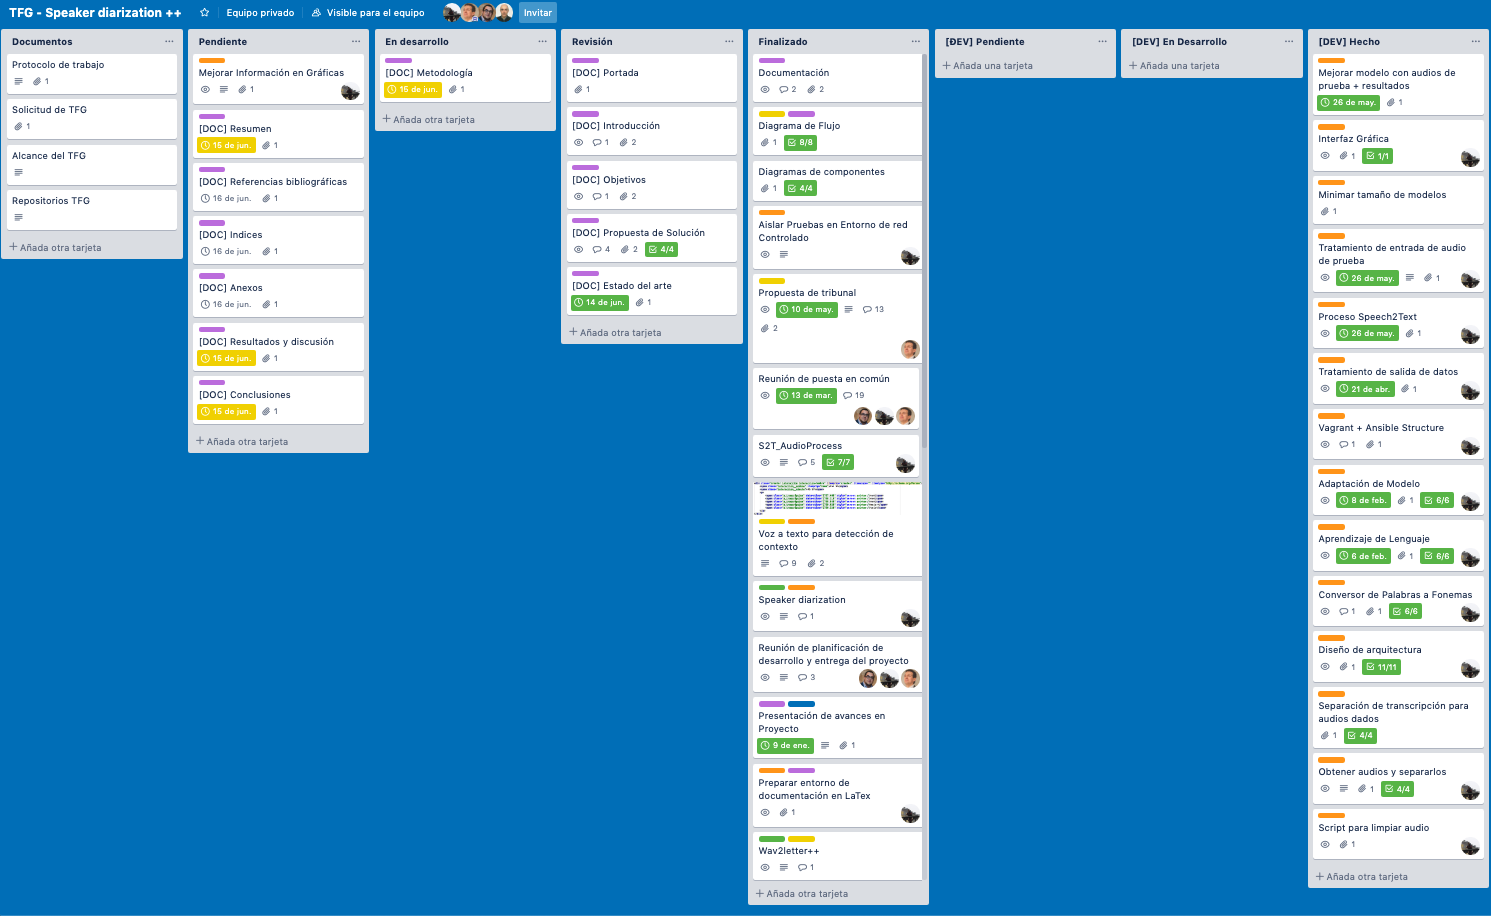
\includegraphics[width=0.7\textwidth]{trello}
    \caption{Tablero de Trello del proyecto.}
    \label{img:trello}
\end{figure}

\section{Planificación}
El proyecto tuvo una \textbf{planificación inicial} de 300 horas de trabajo que se dividieron en: Investigación (30 horas), Diseño y Análisis de la Solución (65 horas), Implementación de la Solución (150 horas), Validación de la Solución (15 horas) y Documentación (40 horas).

Conforme el proyecto fue avanzando, la estimación inicial se incumplió teniendo así un reparto de horas de la siguiente forma: Investigación (77,50 horas), Diseño y Análisis de la Solución (26,74 horas), Implementación de la Solución (303,58 horas), Validación de la Solución (34,12 horas) y Documentación (142,78 horas).

\begin{table}[H]
    \centering
    \resizebox{\textwidth}{!}{%
    \begin{tabular}{|l|c|c|c|c|c|c|}
        \hline
        \textbf{Tareas principales} & \multicolumn{1}{l|}{\textbf{Tiempo estimado {[}h{]}}} & \multicolumn{1}{l|}{\textbf{Total tiempo estimado {[}h{]}}} & \multicolumn{1}{l|}{\textbf{Tiempo dedicado {[}h{]}}} & \multicolumn{1}{l|}{\textbf{Total tiempo dedicado {[}h{]}}} & \multicolumn{1}{l|}{\textbf{Diferencia {[}h{]}}} & \multicolumn{1}{l|}{\textbf{Diferencia Total {[}h{]}}} \\ \hline
        \textbf{Investigación} & 30 &  & 77,50 &  & \cellcolor[HTML]{FFCCC9}+47,5 & \cellcolor[HTML]{FFCCC9} \\ \cline{1-2} \cline{4-4} \cline{6-6}
        \textbf{Diseño y Análisis de Solución} & 65 &  & 26,74 &  & \cellcolor[HTML]{9AFF99}{\color[HTML]{333333} -38,26} & \cellcolor[HTML]{FFCCC9} \\ \cline{1-2} \cline{4-4} \cline{6-6}
        \textbf{Implementación/Desarrollo} & 150 &  & 303,58 &  & \cellcolor[HTML]{FFCCC9}+153,58 & \cellcolor[HTML]{FFCCC9} \\ \cline{1-2} \cline{4-4} \cline{6-6}
        \textbf{Validación} & 15 &  & 34,12 &  & \cellcolor[HTML]{FFCCC9}+19,12 & \cellcolor[HTML]{FFCCC9} \\ \cline{1-2} \cline{4-4} \cline{6-6}
        \textbf{Documentación} & 40 & \multirow{-5}{*}{300} & 142,78 & \multirow{-5}{*}{584,72} & \cellcolor[HTML]{FFCCC9}{\color[HTML]{333333} +102,78} & \multirow{-5}{*}{\cellcolor[HTML]{FFCCC9}+284,72} \\ \hline
    \end{tabular}%
    }
    \caption{Comparativa de horas estimadas y horas dedicadas al desarrollo del proyecto.}
    \label{tab:horas}
\end{table}

Como observamos en la \autoref{tab:horas} existe un gran descompensación entre las horas planificadas y las horas dedicadas (más de 284 horas). Esta descompensación se basa en el crecimiento del proyecto a medida que se ha ido desarrollando ya que se deseaban cumplir todos los objetivos marcados.

Este registro de tiempo se ha realizado utilizando la herramienta \textbf{Harvest}\cite{harvest}. Este software en línea permite registrar el tiempo de trabajo por cada tarea definida anteriormente en Trello. Por tanto, una vez acabado el proyecto se ha podido estudiar el tiempo dedicado en cada una de las tareas definidas.

\section{Gestión de código fuente}
El código fuente del proyecto se ha gestionado a través de repositorios privados de códigos en la plataforma \textbf{GitHub}\cite{github}. GitHub es una plataforma para almacenar proyectos utilizando el sistema de control de versiones \textbf{Git}\cite{Somasundaram2013}. Utilizar un sistema de control de versiones facilita las tareas de mantenimiento del código ya que cada versión que se genere del proyecto se almacenará estando siempre disponible.

Para este proyecto se han creado nueve \textbf{repositorios}: Un repositorio general que contiene a los demás repositorios del proyecto y al código fuente encargado del despliegue de la infraestructura de ejecución, y a ocho repositorios que se corresponden con los componentes del sistema explicados en la \autoref{subsec:arquitectura_sistema}. Estos repositorios de componentes contendrán el código fuente e información de despliegue en contenedores.

El repositorio principal está conectado a los repositorios de los componentes con \textit{Submódulos}. Esto permite que aunque exista un repositorio principal, se puedan mantener un control de versiones de cada componente de forma independiente.

De manera adicional y para crear una conexión normalizada entre la gestión de tareas y las gestión de versiones se ha utilizado el modelo de ramificaciones \textbf{GitFlow}. Este modelo se basa en el uso de las ramas en Git para gestionar las versiones en desarrollo o completadas. Las distintas ramas existentes son:
\begin{itemize}
    \item Rama \textit{master}: Rama principal donde se encuentran versiones del proyecto totalmente funcionales.
    \item Rama \textit{develop}: Rama de trabajo donde se encuentra el código que formará una versión que posteriormente se trasladará a \textit{master}.
    \item Ramas tipo \textit{feature}: Ramas que parten de la rama \textit{develop} y se utilizan para desarrollar una determinada característica de la aplicación. Cuando se termine el trabajo, esta rama se fusionará con \textit{develop} de nuevo. 
\end{itemize}
Aunque existen ramas de tipos \textit{hotfix} y \textit{release} no se han utilizado debido a que el proyecto no lo requería.

En este proyecto se ha trabajado siguiendo un protocolo con las herramientas antes comentadas: Cuando una tarea esta \textit{[Dev] Pendiente} y se empieza a desarrollar, su respectiva tarjeta en Trello se mueve a la columna \textit{[Dev] En desarrollo}. En este momento se crea una rama \textit{feature} en el repositorio del proyecto correspondiente. Una vez la tarea se ha finalizado, la tarjeta de Trello pasa a la columna \textit{[Dev] Finalizado} y la rama creada se fusiona con la rama \textit{develop} resolviendo algunos conflictos que puedan haber sucedido.

Los repositorios con los enlaces a GitHub son:
\begin{itemize}
    \item \textbf{S2T}: \href{https://github.com/pamamu/S2T}{https://github.com/pamamu/S2T}
    \item \textbf{S2T\_AudioProcess}: \href{https://github.com/pamamu/S2T_AudioProcess}{https://github.com/pamamu/S2T\_AudioProcess}
    \item \textbf{S2T\_G2P}: \href{https://github.com/pamamu/S2T_G2P}{https://github.com/pamamu/S2T\_G2P}
    \item \textbf{S2T\_GetAudioTrans}: \href{https://github.com/pamamu/S2T_GetAudiosTrans}{https://github.com/pamamu/S2T\_GetAudiosTrans}
    \item \textbf{S2T\_MainController}: \href{https://github.com/pamamu/S2T_MainController}{https://github.com/pamamu/S2T\_MainController}
    \item \textbf{S2T\_SPHINXBASE}: \href{https://github.com/pamamu/S2T_SPHINXBASE}{https://github.com/pamamu/S2T\_SPHINXBASE}
    \item \textbf{S2T\_SRILM}: \href{https://github.com/pamamu/S2T_SRILM}{https://github.com/pamamu/S2T\_SRILM}
    \item \textbf{S2T\_Speech2Text}: \href{https://github.com/pamamu/S2T_Speech2Text}{https://github.com/pamamu/S2T\_Speech2Text}
    \item \textbf{S2T\_Training}: \href{https://github.com/pamamu/S2T_Training}{https://github.com/pamamu/S2T\_Training}
\end{itemize}

De manera adicional se ha creado un repositorio para almacenar la documentación realizada en \LaTeX: \href{https://github.com/pamamu/S2T_OfficialDocumentation}{https://github.com/pamamu/S2T\_OfficialDocumentation}.


\end{document}

\chapter{Implementación y desarrollo}
Lorem ipsum dolor sit amet, consectetur adipiscing elit, sed eiusmod tempor incidunt ut labore et dolore magna aliqua. Ut enim ad minim veniam, quis nostrud exercitation ullamco laboris nisi ut aliquid ex ea commodi consequat. Quis aute iure reprehenderit in voluptate velit esse cillum dolore eu fugiat nulla pariatur. Excepteur sint obcaecat cupiditat non proident, sunt in culpa qui officia deserunt mollit anim id est laborum.

\documentclass[../main.tex]{subfiles}
\begin{document}

\chapter{Conclusiones y trabajos futuros}\label{ch:conclusiones}
\section{Conclusiones}\label{sec:conclusiones}
Este trabajo se puede resumir en dos palabras: complejo e innovador.

\textbf{Complejo} debido a la gran cantidad de estudios e investigaciones que se han realizado tanto del entorno de las herramientas de reconocimiento de voz como del sistema elegido, CMUSphinx. El reconocimiento de la voz humana es un problema difícil de resolver y es por ello que las grandes empresas líderes en I+D+i estén dedicando muchas horas y recursos en el desarrollo y mejora de estos sistemas.

\textbf{Innovador} porque no existía hasta la fecha un sistema tal y como el que se ha desarrollado y presentado en este documento. Existen multitud de herramientas relacionadas con el reconocimiento de voz, como se ha explicado en el \autoref{ch:estado_arte}, pero ninguna de ellas permite funcionalidades como aumento del vocabulario y mejora del modelo tanto acústico como fonético. Además este proyecto se ha desarrollado bajo las premisas del Software Libre publicándolo con una licencia permisiva (Licencia MIT).

Con este trabajo se han investigado y desarrollado nuevas formas de despliegue de aplicaciones orientadas al reconocimiento de voz. Hasta donde conoce el autor, no existía un sistema de reconocimiento de voz modular (dividido en microservicios) y con la capacidad de desplegarse tanto localmente como distribuidamente.

El autor de este trabajo espera que después de haber conocido este proyecto, el mundo del reconocimiento de la voz humana sea algo más conocido y que la investigación y el desarrollo realizado pueda servir a otros para desarrollar sus propios sistema de \textit{Speech to Text} (Reconocimiento de Voz). Queda mucho trabajo por hacer en este campo y usted, lector de esta memoria, puede contribuir al crecimiento de esta rama de la lingüística computacional.

Volviendo al punto de los Objetivos, en la \autoref{tab:obj-terminados} se analizan los objetivos y el estado de cumplimiento después del desarrollo del proyecto.

\begin{table}[H]
    \centering
    \resizebox{\textwidth}{!}{%
    \begin{tabular}{m{12cm} c}
    \hline
    \multicolumn{1}{|c|}{\textbf{Objetivo}} & \multicolumn{1}{c|}{\textbf{Consecución}} \\\hline
    \textbf{O1} - Diseño e implementación de un sistema de tratamiento de audio que sea capaz de transcribir a texto ficheros de audio indexando cada una de las palabras que son reconocidas. & 80\% \\[1cm]
    \textbf{O2} - Tratamiento del audio de entrada para que se normalicen las características del audio con el que mejorar el sistema. & 90\% \\ [1cm]
    \textbf{O3} - Aprendizaje de palabras nuevas que se adapten al caso de uso en el que se vaya a aplicar este sistema. & 100\% \\[1cm]
    \textbf{O4} - Mejora del modelo de lenguaje que se utiliza para determinar la salida del sistema de transcripción de voz a texto. & 100\% \\[1cm]
    \textbf{O5} - Mejora del modelo acústico que identifica en una señal de audio las palabras pronunciadas por el hablante. & 80\% \\[1cm]
    \textbf{O6} - Interfaz que permita al usuario utilizar todos los servicios del sistema sin necesidad de procesos tediosos de instalación y configuración. & 90\% \\[1cm]
    \textbf{O7} - Ninguna de las herramientas utilizadas tendrán un coste por dicha utilización y los 
    \textit{frameworks} serán de código abierto. & 100\% \\ 
    \textbf{O8} - Transcripciones con más de un 80\% de coincidencia sobre la transcripción real. & No \\[1cm] \hline
    \end{tabular}%
    }
    \caption{Relación de consecución de objetivos.}
    \label{tab:obj-terminados}
\end{table}

A continuación se analizarán los objetivos que no tienen una consecución del 100\%, como se muestra en la \nameref{tab:obj-terminados}
\begin{itemize}
    \item \textbf{O1} - Aunque el diseño y la implementación del sistema se ha completado, no se ha realizado una indexación de las palabras reconocidas, sino que se ha almacenado solamente su marca temporal.
    \item \textbf{O2} - Aunque se realizan filtrados del audio, en ficheros con alto nivel de ruido no se llega a eliminar al 100\% todo el sonido que no es voz humana.
    \item \textbf{O5} - El sistema realiza una mejora basada en la adaptación de un modelo acústico exitente. No se realiza un entrenamiento del modelo acústico.
    \item \textbf{O6} - La interfaz procesa la entrada y devuelve una salida, aunque este proceso se realiza de forma síncrona bloqueando la navegación del usuario.
    \item \textbf{O8} - Las transcripciones no llegan al 80\% de coincidencia ni antes del entrenamiento (con modelos base), ni después de horas de entrenamiento.
\end{itemize}

\subsection{Conclusión Personal}


\section{Trabajos futuros}\label{sec:trabajos_futuros}
Según el informe anual de tecnologías emergentes de 2019 (Gartner Hype Cycle)\cite{Gartner2018}, en 2022 el 70\% de las empresas estarán experimentando con tecnologías inmersivas como plataformas de conversación, que incluyen desde  asistentes personales a chatbots. La mayoría de estas tecnologías pueden utilizar el sistema propuesto en este trabajo para realizar el reconocimiento de voz. Por lo que se proponen los siguientes trabajos futuros:

\subsection{Aumento del entrenamiento de audios}
Como se ha explicado en la \autoref{sec:val-train}, cuánto mayor es el entrenamiento, mayor la calidad de las transcripciones con respecto a la transcripción original. Por lo tanto, para mejorar el rendimiento del sistema de reconocimiento de voz se debe aumentar el entrenamiento del sistema mediante audios de larga duración con sus correspondientes transcripciones (tan buenas como sean posibles).

\subsection{Detección de hablantes - Speaker Diarization}
Aunque inicialmente este caso de uso se incluía en el dominio de este trabajo, se descartó debido a la carga de tiempo planteada. Utilizando herramientas de segmentación y clasificación se pueden buscar patrones tanto en las características de la voz como en el modelo de lenguaje utilizado para diferenciar hablantes en un audio. 

Se investigó la herramienta PyAudioAnalysis\cite{Giannakopoulos2015} cómo una posible aproximación.

\subsection{Detección de sentimientos}
Esta funcionalidad puede incluirse en el sistema sin demasiada dificultad y sería bastante interesante que se identificaran emociones en la voz de las personas del audio. Como en el caso anterior, no solamente con las características de la voz sino por la forma de hablar.

\subsection{API Rest y Despliegue en la nube}
Una de las funcionalidades que no ofrece el presente sistema es una API Rest de conexión con el sistema para poder realizar operaciones sin necesidad de operar a través de la interfaz web. Esto permitirá la conexión de aplicaciones con este sistema, haciéndolo así más intregable incluso.

Esta API Rest, junto con el sistema completo, se pondría en un servicio de Cloud Computing para estar disponible a través de internet.

\end{document}


%%%%%%%%%%%%%%%%%%%%%%%%%%%%%%%%%%
%%%%%%%%%%% ANEXOS %%%%%%%%%%%%%%%
%%%%%%%%%%%%%%%%%%%%%%%%%%%%%%%%%%
\appendix
\clearpage
\appendixpage
\addappheadtotoc

\chapter{Ejemplo de anexo}
Si no se desea incluir anexos, sólo hay que borrar este capítulo.
\par
Lorem ipsum dolor sit amet, consectetur adipiscing elit, sed eiusmod tempor
incidunt ut labore et dolore magna aliqua. Ut enim ad minim veniam, quis nostrud exercitation ullamco laboris nisi ut aliquid ex ea commodi consequat. Quis aute iure reprehenderit in voluptate velit esse cillum dolore eu fugiat nulla pariatur. Excepteur sint obcaecat cupiditat non proident, sunt in culpa qui officia deserunt mollit anim id est laborum.\\


\pagebreak
%%%%%%%%%%%%%%%%%%%%%%%%%%%%%%%%%%
%%%%%%%% bibliografia %%%%%%%%%%%%
%%%%%%%%%%%%%%%%%%%%%%%%%%%%%%%%%%

\thispagestyle{empty}
\pagestyle{empty}
\addcontentsline{toc}{chapter}{Bibliografía}
\bibliographystyle{unsrt}
\bibliography{library.bib}
\end{document}
